\documentclass[12pt,twoside]{article}
\usepackage[dvipsnames]{xcolor}
\usepackage{tikz,graphicx,amsmath,amsfonts,amscd,amssymb,bm,cite,epsfig,epsf,url}
\usepackage[hang,flushmargin]{footmisc}
\usepackage[colorlinks=true,urlcolor=blue,citecolor=blue]{hyperref}
\usepackage{amsthm,multirow,wasysym,appendix}
\usepackage{array,subcaption} 
% \usepackage[small,bf]{caption}
\usepackage{bbm}
\usepackage{pgfplots}
\usetikzlibrary{spy}
\usepgfplotslibrary{external}
\usepgfplotslibrary{fillbetween}
\usetikzlibrary{arrows,automata}
\usepackage{thmtools}
\usepackage{blkarray} 
\usepackage{textcomp}
\usepackage[left=0.8in,right=1.0in,top=1.0in,bottom=1.0in]{geometry}
\usepackage{pifont}
\usepackage{tikz-qtree}

%% Probability operators and functions
%
% \def \P{\mathrm{P}}
\def \P{\mathrm{P}}
\def \E{\mathrm{E}}
\def \Var{\mathrm{Var}}
\let\var\Var
\def \Cov {\mathrm{Cov}} \let\cov\Cov
\def \MSE {\mathrm{MSE}} \let\mse\MSE
\def \sgn {\mathrm{sgn}}
\def \R {\mathbb{R}}
\def \C {\mathbb{C}}
\def \N {\mathbb{N}}
\def \Z {\mathbb{Z}}
\def \cV {\mathcal{V}}
\def \cS {\mathcal{S}}

\newcommand{\RR}{\ensuremath{\mathbb{R}}}

\DeclareMathOperator*{\argmin}{arg\,min}
\DeclareMathOperator*{\argmax}{arg\,max}
\newcommand{\red}[1]{\textcolor{red}{#1}}
\newcommand{\blue}[1]{\textcolor{blue}{#1}}
\newcommand{\green}[1]{\textcolor{ForestGreen}{ #1}}
\newcommand{\fuchsia}[1]{\textcolor{RoyalPurple}{ #1}}



%
%% Probability distributions
%
%\def \Bern    {\mathrm{Bern}}
%\def \Binom   {\mathrm{Binom}}
%\def \Exp     {\mathrm{Exp}}
%\def \Geom    {\mathrm{Geom}}
% \def \Norm    {\mathcal{N}}
%\def \Poisson {\mathrm{Poisson}}
%\def \Unif    {\mathrm {U}}
%
\DeclareMathOperator{\Norm}{\mathcal{N}}

\newcommand{\bdb}[1]{\textcolor{red}{#1}}

\newcommand{\ml}[1]{\mathcal{ #1 } }
\newcommand{\wh}[1]{\widehat{ #1 } }
\newcommand{\wt}[1]{\widetilde{ #1 } }
\newcommand{\conj}[1]{\overline{ #1 } }
\newcommand{\rnd}[1]{\tilde{ #1 } }
\newcommand{\rv}[1]{ \rnd{ #1}  }
\newcommand{\rM}{\rnd{ m}  }
\newcommand{\rx}{\rnd{ x}  }
\newcommand{\ry}{\rnd{ y}  }
\newcommand{\rz}{\rnd{ z}  }
\newcommand{\ra}{\rnd{ a}  }
\newcommand{\rb}{\rnd{ b}  }
\newcommand{\rt}{\rnd{ t}  }
\newcommand{\rs}{\rnd{ s}  }


\newcommand{\rpc}{\widetilde{ pc}  }
\newcommand{\rndvec}[1]{\vec{\rnd{#1}}}

\def \cnd {\, | \,}
\def \Id { I }
\def \J {\mathbf{1}\mathbf{1}^T}

\newcommand{\op}[1]{\operatorname{#1}}
\newcommand{\setdef}[2]{ := \keys{ #1 \; | \; #2 } }
\newcommand{\set}[2]{ \keys{ #1 \; | \; #2 } }
\newcommand{\sign}[1]{\op{sign}\left( #1 \right) }
\newcommand{\trace}[1]{\op{tr}\left( #1 \right) }
\newcommand{\tr}[1]{\op{tr}\left( #1 \right) }
\newcommand{\inv}[1]{\left( #1 \right)^{-1} }
\newcommand{\abs}[1]{\left| #1 \right|}
\newcommand{\sabs}[1]{| #1 |}
\newcommand{\keys}[1]{\left\{ #1 \right\}}
\newcommand{\sqbr}[1]{\left[ #1 \right]}
\newcommand{\sbrac}[1]{ ( #1 ) }
\newcommand{\brac}[1]{\left( #1 \right) }
\newcommand{\bbrac}[1]{\big( #1 \big) }
\newcommand{\Bbrac}[1]{\Big( #1 \Big)}
\newcommand{\BBbrac}[1]{\BIG( #1 \Big)}
\newcommand{\MAT}[1]{\begin{bmatrix} #1 \end{bmatrix}}
\newcommand{\sMAT}[1]{\left(\begin{smallmatrix} #1 \end{smallmatrix}\right)}
\newcommand{\sMATn}[1]{\begin{smallmatrix} #1 \end{smallmatrix}}
\newcommand{\PROD}[2]{\left \langle #1, #2\right \rangle}
\newcommand{\PRODs}[2]{\langle #1, #2 \rangle}
\newcommand{\der}[2]{\frac{\text{d}#2}{\text{d}#1}}
\newcommand{\pder}[2]{\frac{\partial#2}{\partial#1}}
\newcommand{\derTwo}[2]{\frac{\text{d}^2#2}{\text{d}#1^2}}
\newcommand{\ceil}[1]{\lceil #1 \rceil}
\newcommand{\Imag}[1]{\op{Im}\brac{ #1 }}
\newcommand{\Real}[1]{\op{Re}\brac{ #1 }}
\newcommand{\norm}[1]{\left|\left| #1 \right|\right| }
\newcommand{\norms}[1]{ \| #1 \|  }
\newcommand{\normProd}[1]{\left|\left| #1 \right|\right| _{\PROD{\cdot}{\cdot}} }
\newcommand{\normTwo}[1]{\left|\left| #1 \right|\right| _{2} }
\newcommand{\normTwos}[1]{ \| #1  \| _{2} }
\newcommand{\normZero}[1]{\left|\left| #1 \right|\right| _{0} }
\newcommand{\normTV}[1]{\left|\left| #1 \right|\right|  _{ \op{TV}  } }% _{\op{c} \ell_1} }
\newcommand{\normOne}[1]{\left|\left| #1 \right|\right| _{1} }
\newcommand{\normOnes}[1]{\| #1 \| _{1} }
\newcommand{\normOneTwo}[1]{\left|\left| #1 \right|\right| _{1,2} }
\newcommand{\normF}[1]{\left|\left| #1 \right|\right| _{\op{F}} }
\newcommand{\normLTwo}[1]{\left|\left| #1 \right|\right| _{\ml{L}_2} }
\newcommand{\normNuc}[1]{\left|\left| #1 \right|\right| _{\ast} }
\newcommand{\normOp}[1]{\left|\left| #1 \right|\right|  }
\newcommand{\normInf}[1]{\left|\left| #1 \right|\right| _{\infty}  }
\newcommand{\proj}[1]{\mathcal{P}_{#1} \, }
\newcommand{\diff}[1]{ \, \text{d}#1 }
\newcommand{\vc}[1]{\boldsymbol{\vec{#1}}}
\newcommand{\rc}[1]{\boldsymbol{#1}}
\newcommand{\vx}{\vec{x}}
\newcommand{\vy}{\vec{y}}
\newcommand{\vz}{\vec{z}}
\newcommand{\vu}{\vec{u}}
\newcommand{\vv}{\vec{v}}
\newcommand{\vb}{\vec{\beta}}
\newcommand{\va}{\vec{\alpha}}
\newcommand{\vaa}{\vec{a}}
\newcommand{\vbb}{\vec{b}}
\newcommand{\vg}{\vec{g}}
\newcommand{\vw}{\vec{w}}
\newcommand{\vh}{\vec{h}}
\newcommand{\vbeta}{\vec{\beta}}
\newcommand{\valpha}{\vec{\alpha}}
\newcommand{\vgamma}{\vec{\gamma}}
\newcommand{\veta}{\vec{\eta}}
\newcommand{\vnu}{\vec{\nu}}
\newcommand{\rw}{\rnd{w}}
\newcommand{\rvnu}{\vc{\nu}}
\newcommand{\rvv}{\rndvec{v}}
\newcommand{\rvw}{\rndvec{w}}
\newcommand{\rvx}{\rndvec{x}}
\newcommand{\rvy}{\rndvec{y}}
\newcommand{\rvz}{\rndvec{z}}
\newcommand{\rvX}{\rndvec{X}}


\newtheorem{theorem}{Theorem}[section]
% \declaretheorem[style=plain,qed=$\square$]{theorem}
\newtheorem{corollary}[theorem]{Corollary}
\newtheorem{definition}[theorem]{Definition}
\newtheorem{lemma}[theorem]{Lemma}
\newtheorem{remark}[theorem]{Remark}
\newtheorem{algorithm}[theorem]{Algorithm}

% \theoremstyle{definition}
%\newtheorem{example}[proof]{Example}
\declaretheorem[style=definition,qed=$\triangle$,sibling=definition]{example}
\declaretheorem[style=definition,qed=$\bigcirc$,sibling=definition]{application}

%
%% Typographic tweaks and miscellaneous
%\newcommand{\sfrac}[2]{\mbox{\small$\displaystyle\frac{#1}{#2}$}}
%\newcommand{\suchthat}{\kern0.1em{:}\kern0.3em}
%\newcommand{\qqquad}{\kern3em}
%\newcommand{\cond}{\,|\,}
%\def\Matlab{\textsc{Matlab}}
%\newcommand{\displayskip}[1]{\abovedisplayskip #1\belowdisplayskip #1}
%\newcommand{\term}[1]{\emph{#1}}
%\renewcommand{\implies}{\;\Rightarrow\;}



\begin{document}

\begin{center}
{\large{\textbf{Homework 10}} } \vspace{0.2cm}\\
Due Apr 16 at 11 pm
\\
\end{center}
Unless stated otherwise, justify any answers you give.
You can work in groups, but each
student must write their own solution based on their own
understanding of the problem.

When uploading your homework to Gradescope you will have to
select the relevant pages for each question.  Please submit each
problem on a separate page (i.e., 1a and~1b can be on the same page but 1
and 2 must be on different pages).  We understand that this may be
cumbersome but this is the best way for the grading team to grade your
homework assignments and provide feedback in a timely manner.  Failure
to adhere to these guidelines may result in a loss of points.
Note that it may take some time to
select the pages for your submission.  Please plan accordingly.  We
suggest uploading your assignment at least 30 minutes before the deadline
so you will have ample time to select the correct pages for your
submission.  If you are using \LaTeX, consider using the minted or
listings packages for typesetting code.  
\\

\begin{enumerate}

\item (Numerical rank) 
The rank of a matrix is not numerically stable, in the sense that most perturbations will render the matrix full rank. A more stable definition of rank is the numerical rank
\begin{align}
\op{rank}_{\op{num}} (M) := \min_{ \normF{L-M} \leq \epsilon }\op{rank} (L),
\end{align}
where $\epsilon$ is a fixed constant. Explain how to compute the numerical rank and why your method is guaranteed to work.
\begin{itemize}
    \color{blue}
    \item as we showed in textbook section 11.6.4 the optimal rank r approximation of for an arbitrary matrix $M$ in terms of Frobenius norm is the rank approximation of M obtained form its svd truncated to r dimensions.  
    \item thus we can just $Rank_{num}(M)=argmin_{r\in [1,n]}\mathbb{I}(||L_{\text{svd rank r}} -M||_{F}\leq \epsilon)$
    \item that is we can the lowest value of r, such that the error of our rank r approximation ac hived by the truncated svd at rank r is less than $\epsilon$
    \item this will always work as we showed in textbook section 11.6.4 the optimal rank r approximation of for an arbitrary matrix $M$ in terms of Frobenius norm is the rank approximation of M obtained form its svd truncated to r dimensions. So in other words each of these Truncated SCD estimation is optimal in it's dimension, so the first dimension that has an error within the bounds we want, will equal the numerical rank.   
\end{itemize}


\newpage
\item (Exact matrix completion) Find the matrix with the lowest possible rank that is compatible with the revealed entries:
\begin{align}
D:=\MAT{ ? & ? & 2 & 0 \\ 2 & 2 & 3 & ? \\ 2 & 3 & 4 & -2 \\ 2 & 4 & ? & -3}.
\end{align}
\begin{itemize}
    \color{blue}
    \item two vectors $v_1,v_2 $are linearly dependent if there exists $\alpha \in \mathbb{Z}:\alpha v_1=v_2 $
    \item we can see that row 1 is linearly independent for rows 3 and 4, as row 1 has a zero element in position 4 while the others have no zero elements in position 4.  so the matrix must at least have rank 2.
    \item additionally we can see that row 2 and 3 must be linearly independent as there first element is the same but the second differs, meaning there is no scalar that will equate them. so the matrix must at least have rank 3. 
    \item so the matrix \begin{align}
D:=\MAT{ \frac{3}{2} & \frac{3}{2} & 2 & 0 \\ 2 & 2 & 3 & 0 \\ 2 & 3 & 4 & -2 \\ 2 & 4 & x & -3}.
\end{align}
will always have rank 3 regardless of the value of x. 
\end{itemize}


\newpage
\item (Topic modeling) Topic modeling aims to learn the thematic structure of a text corpus automatically. In this example, we take six newspaper articles and compute the frequency of a list of words in each of them. The following matrix contains the counts for each word and article. Each entry contains the number of times that the word in column $j$ is mentioned in the article corresponding to row $i$. 
\begin{align*}
D: = \quad &
\begin{blockarray}{cccccccccc}
  \text{singer} & \text{GDP} & \text{senate} & \text{election} & \text{vote} &  \text{stock}& \text{concert} & \text{market} & \text{band} & Articles\\
\begin{block}{(ccccccccc)c}
6 & 1 & 1 & 0 & 0 & 1 & 9 & 0 & 8 & \hspace{0.2cm} \text{a}  \\  
1 & 0 & 9 & 5 & 8 & 1 & 0 & 1 & 0 & \hspace{0.2cm} \text{b}  \\
8 & 1 & 0 & 1 & 0 & 0 & 9 & 1 & 7 & \hspace{0.2cm} \text{c}  \\
0 & 7 & 1 & 0 & 0 & 9 & 1 & 7 & 0 & \hspace{0.2cm} \text{d} \\
0 & 5 & 6 & 7 & 5 & 6 & 0 & 7 & 2 & \hspace{0.2cm} \text{e} \\
1 & 0 & 8 & 5 & 9 & 2 & 0 & 0 & 1 & \hspace{0.2cm} \text{f} \\
\end{block}
\end{blockarray}
\end{align*}
We consider a low-rank topic model, where the counts $D[i,j]$ for word $i$ and article $j$ are approximated by
\begin{align}
D[i,j] \approx \sum_{l=1}^{r} a_{l}[i] b_{l}[j], \qquad 1\leq i \leq 9, 1 \leq j \leq 6.
\end{align} 
Intuitively, each term $ a_{l} b_{l}$ is associated to a different \emph{topic}.
\begin{enumerate}
\item Compute the SVD of the matrix. Based on the results, what do you think should be the number of topics $r$ in the model?
\begin{itemize}
    \color{blue}
\item running svd we get\\ U=\begin{pmatrix}
-0.24393829712528042&0.6448002977980025&-0.075627366399977&-0.19130855482207845&-0.6214699772570458&-0.310134307722709&\\
-0.4652684261311566&-0.23336530085388119&-0.3910529191305769&-0.17848576089994228&0.3634277724210776&-0.642033199944746&\\
-0.24282837792381762&0.673249842902534&-0.08045161573201809&0.18251477917912806&0.6102348215053781&0.2749516019887902&\\
-0.31695292569903044&-0.02756112374203288&0.7723912664051601&-0.5257236028213301&0.16052507478347294&0.006273175611694631&\\
-0.5826212780490041&-0.17885152629367587&0.2818777968804174&0.710753010953324&-0.20961664700092758&-0.0007101082186889429&\\
-0.4744966459010142&-0.2091898117719818&-0.39855023851936294&-0.34158026325652174&-0.19900086906676706&0.6449587900943174&\\
\end{pmatrix}, \\
S=\begin{pmatrix}
23.64220200171002&\\
18.824584089317348&\\
14.231553287814195&\\
3.6298806722218178&\\
2.026293847933214&\\
1.3646644048713166&\\
\end{pmatrix}\\
$V^T=\begin{pmatrix}
-0.18382475024365552&-0.23764891040102576&-0.5092591583743349&-0.38152125947385507&-0.4612820587360942&-0.3386530583769084&-0.19870623729554118&-0.29629711436289&-0.22379659153937045&\\
0.4681243089127919&0.01226399701276458&-0.22468895809321726&-0.14828940660987233&-0.2466927461564794&-0.07055156659710062&0.6286933132976312&-0.05338784662826278&0.49426103515468606&\\
-0.1325913091666302&0.46797765025472665&-0.303540127467414&-0.14442013350564264&-0.37283256493583605&0.5184962784545778&-0.04443081932063035&0.4854269079715824&-0.07047543341184483&\\
-0.057246818399878226&-0.0372171850329591&-0.21805897150625456&0.704556420997905&-0.2612602141439391&-0.41873255325959363&-0.16663566608035346&0.357927709620243&0.22784792366773832&\\
0.6501947450508587&0.031761006822207886&-0.01964265215737209&-0.01724685230881262&0.033722217946216076&-0.2314660099285214&0.0293188833786657&0.3109231116932448&-0.6506214446300755&\\
0.2504150899692159&0.0037950593831049834&-0.6791048823895385&0.20855588684652435&0.4871622413718129&0.2857464460290272&-0.22743406722244086&-0.24045481440974517&0.06384377396068633&\\
-0.46269538124248544&0.03756733013609592&-0.2490278996241302&0.2120828920323084&0.21525207120440273&-0.07608221118143102&0.6876128745940664&-0.00240234075567548&-0.3906001004027777&\\
-0.0853565620357898&-0.7429812998626422&-0.10677231671429628&-0.22676323825248576&0.18393172889546966&0.15467908779191625&0.037594832227059456&0.5539906847712119&0.10860755136952821&\\
-0.13920041967468602&0.4105224835420667&-0.12449562325126362&-0.4183313566506421&0.44774094949748744&-0.5207874540954975&-0.09331836681778834&0.2901776703048665&0.23872855165161316&\\
\end{pmatrix}$
\item the first three singular values of $D$ are much larger than the others so $r=3$ may be prudent. 
\end{itemize}


\item Ideally, we would like the coefficients $a_l[i]$ and $b_l[j]$ to be nonnegative, since a word contributes to the count if it is present, and does not contribute if it isn't, but negative contributions don't make much sense. Why is it difficult for several left or right singular vectors of a matrix to all have nonnegative entries?   
\begin{itemize}
    \color{blue}
    \item the SVD of a matrix is non-unique, but it must have all U and V orthonromal.
    \item but for any two vectors $v_1, v_2$ to be orthogonal it must be the case that $v_1^Tv_2\Sigma_{i=1}^{n}v_1[i]v_2[i]=0$, but this will never be the case for two vectors with all positive entries because the product of any 2 positive numbers will be positive and thus they will have a positive dot product and not be orthogonal.
    \item so the number of non negative orthogonal vectors we can have is pretty limited, and heavily reliant on where the zero is placed. 
    \item so it makes sense that vectors that have mixed positive and negative entries that are orthogonal will be easier to find and give our SVD more flexibility. 
\end{itemize}
\item Fit the low-rank model using nonnegative matrix factorization, which constrains the coefficients $a_l[i]$ and $b_l[j]$ to be nonnegative (we suggest you use the function sklearn.decomposition.NMF from scikit-learn). Set $r$ following your answer to part (a). Report the coefficients and use them to assign each word and article to one or more topics. 
\begin{itemize}
    \color{blue}
    \item fitting this matrix using the described function yields two matrices \\$A=$\begin{pmatrix}
0.01190850692834251&0.005262423033727666&1.5767924927150732&\\
0.9702772685551496&0.0&0.0&\\
0.0&0.00141148508684338&1.6365920643541692&\\
0.0&0.5522651097256783&0.0&\\
0.6933714306020177&0.40956706595414927&0.0&\\
0.9743376648154729&0.0&0.0253259572065022&\\
\end{pmatrix}
\item and $B.T=$\begin{pmatrix}
0.7700893907585723&0.0&4.364729682415467&\\
0.0&12.509289929931949&0.5964143953646323&\\
8.576648468871714&1.2181727627148176&0.26983547595370566&\\
5.834785154380818&2.5551405450073283&0.2870235473861541&\\
8.432054233526953&0.0&0.0&\\
1.1881351761372119&15.002287244919865&0.2742651092207244&\\
0.0&1.1696210286650313&5.596533909991402&\\
0.8030894663548505&13.755338675986385&0.28183604016162983&\\
0.7997879624055215&1.2575899238801933&4.655583607159878&\\
\end{pmatrix}
\item from this i would assign the articles in order as to topics 3, 1, 3, 2, 1, 1, and the words to topics 3, 2, 1, 1, 1, 2, 3, 2, 3
\end{itemize}
\item Build rank-$r$ approximations to $D$ using the SVD and the coefficients from nonnegative matrix factorization. Which model achieves better approximation error in Frobenius norm? Was this to be expected? Does this mean that it is a better model?
\begin{itemize}
    \color{blue}
    \item conducting  this analysis my non negative model got an error of $
4.444581123006968$
\item while my SVD model got an error of $4.3754096254710015$
\item so the SVD model did a bit better this is to be expected, as SVD described above SVD is less restricted in it's approximation of the matrix. 
\item this however does not necessarily mean the model is better, as we are still only testing on a known dataset so we can really say anything about generalization (ie the SVD may be over fitting) and the non-negative model is more inheritable 
\end{itemize}
\end{enumerate}
\newpage
\item (Predicting movie ratings) Fit a low-rank collaborative filtering model for movie rating prediction. Complete the notebook \texttt{collaborative\_filtering\_svd\_question.ipynb}.
\begin{itemize}
    \color{blue}
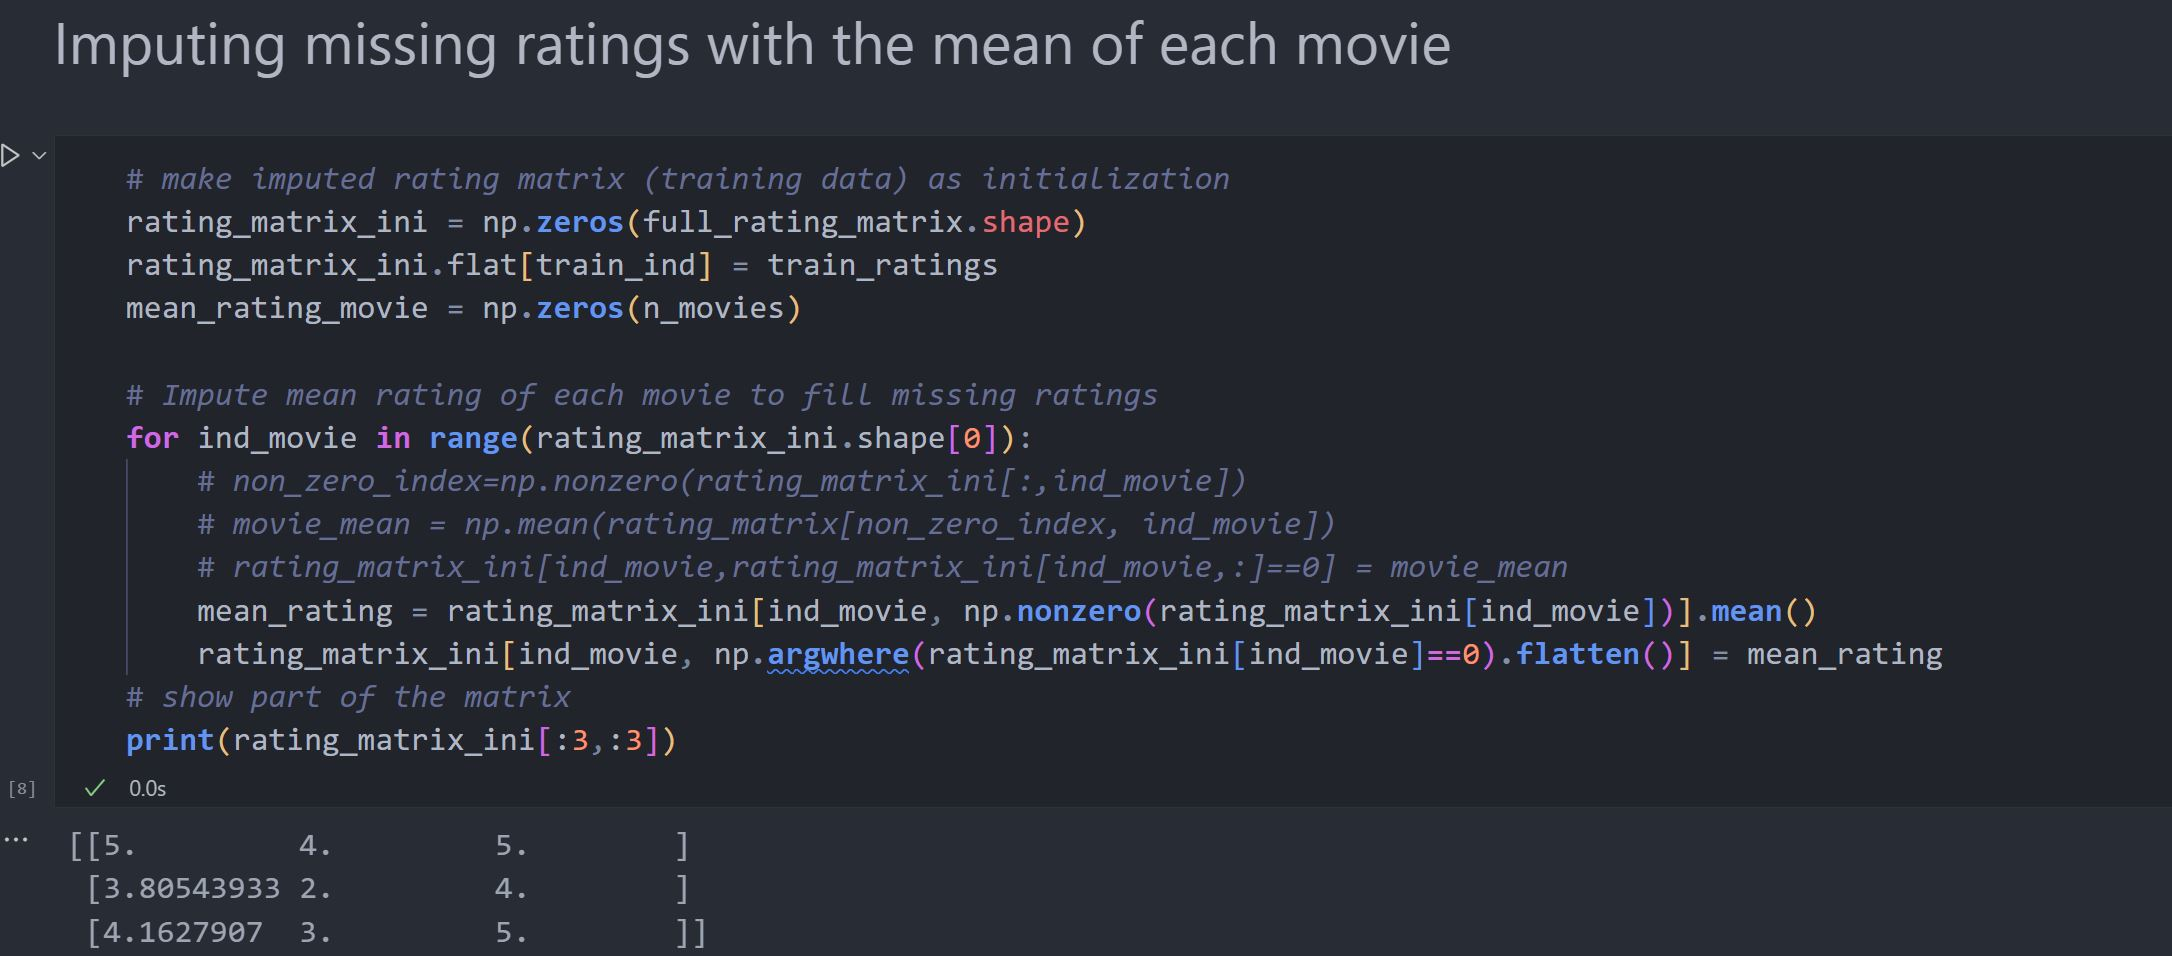
\includegraphics[width=14cm]{homework/homework_10/images/part_a.jpg}\\

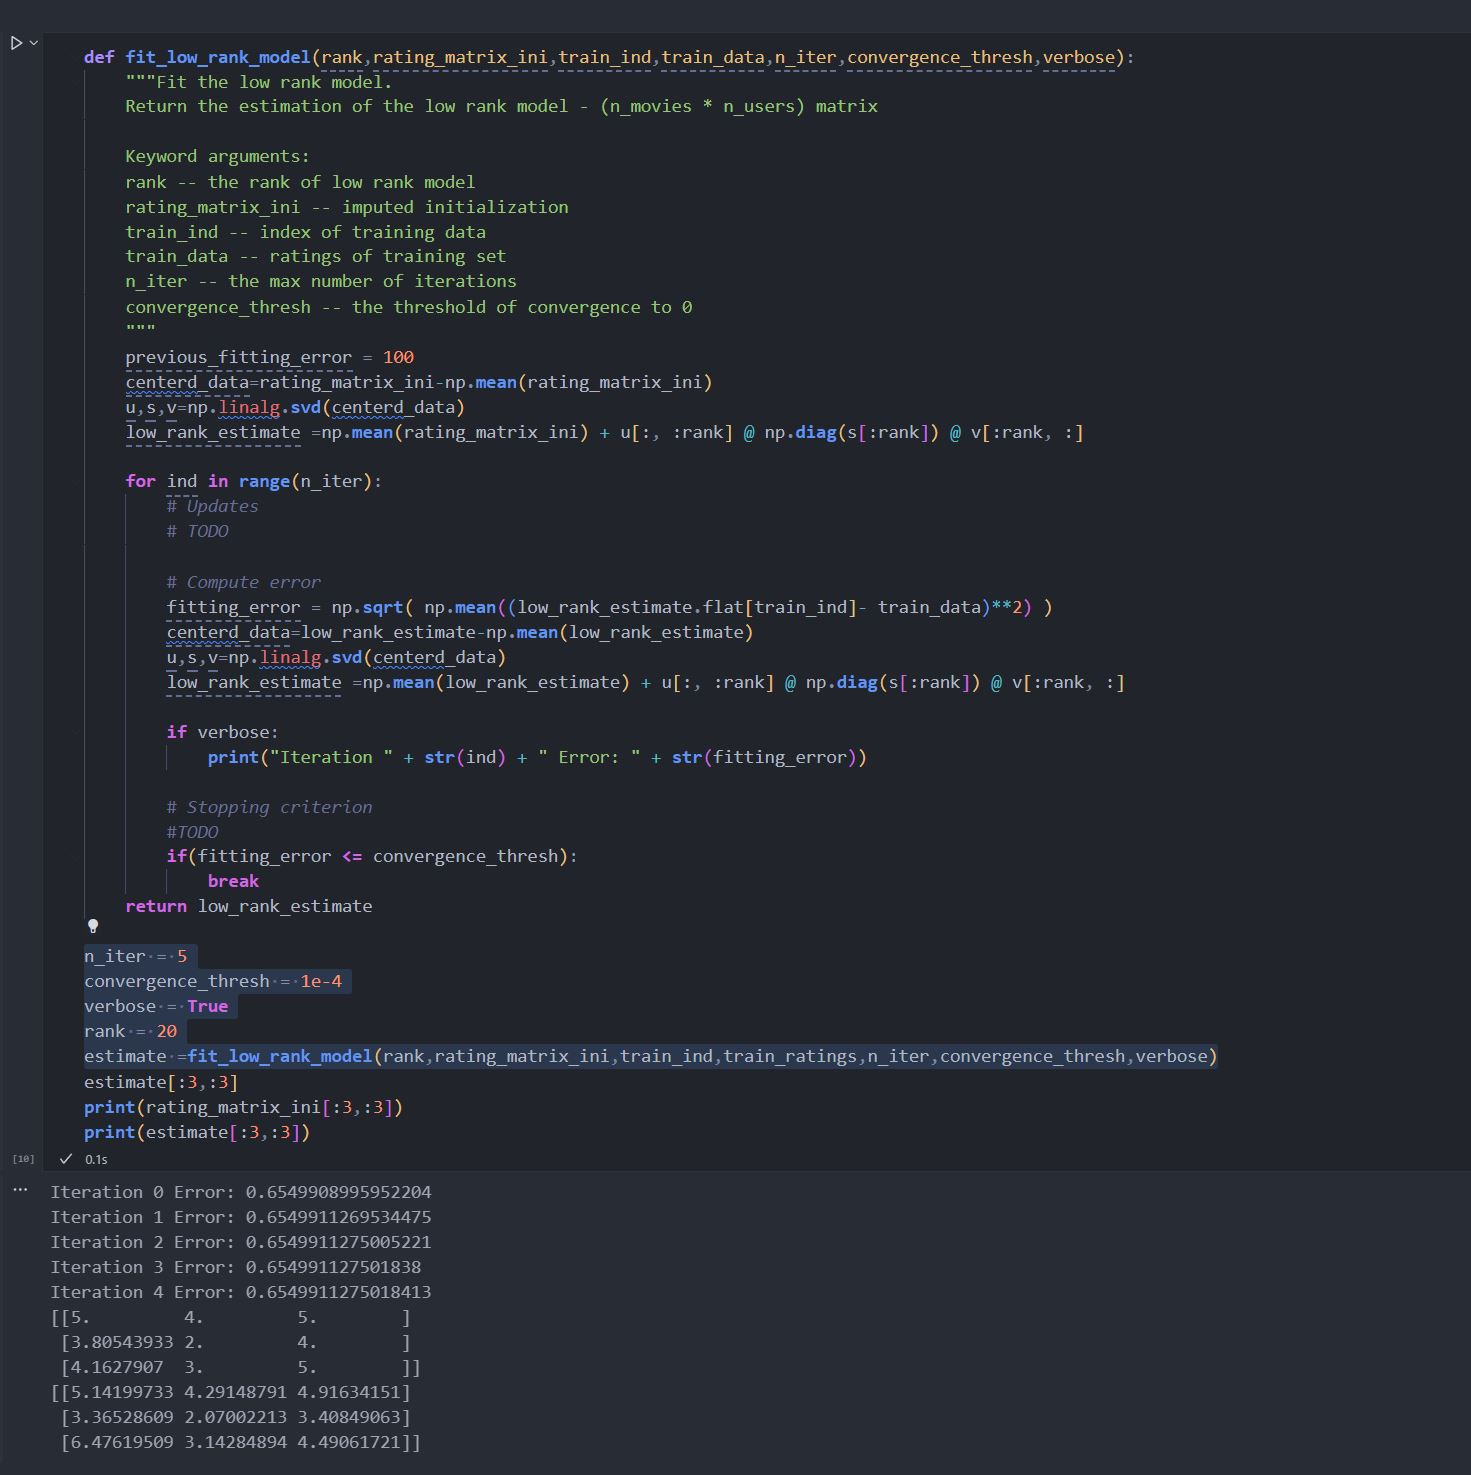
\includegraphics[width=20cm]{homework/homework_10/images/part_b.jpg}
\\
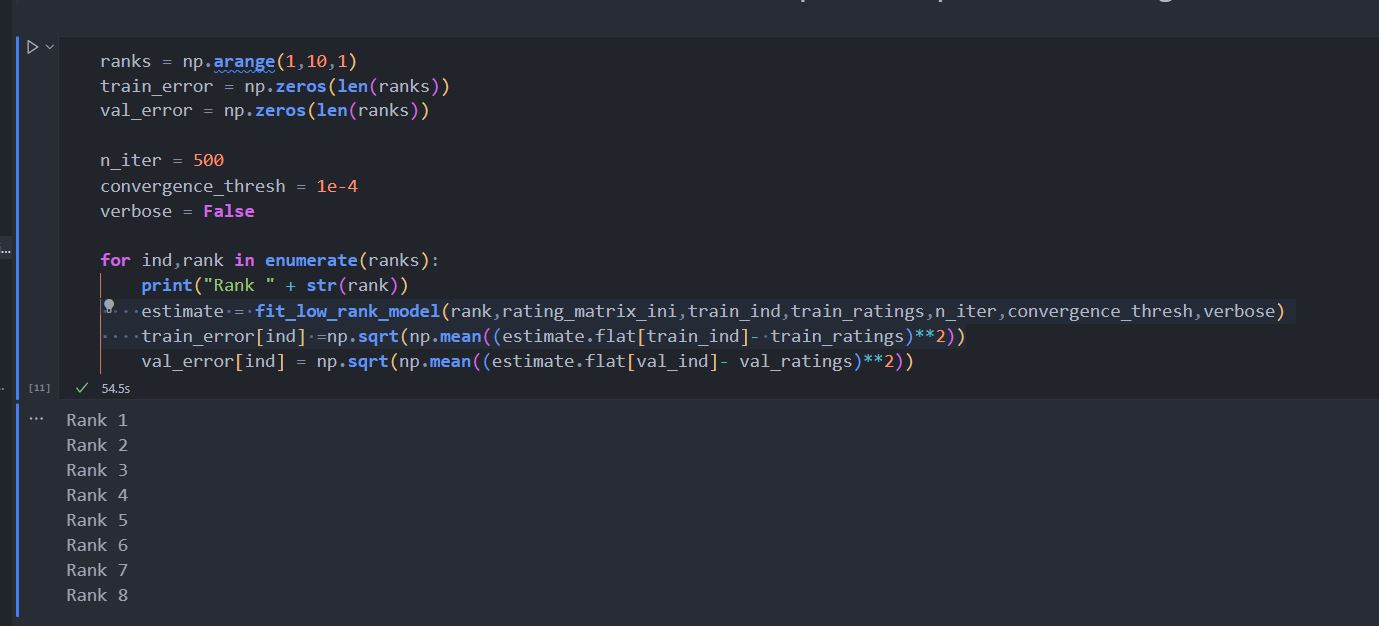
\includegraphics[width=20cm]{homework/homework_10/images/part_c_1.jpg}
\\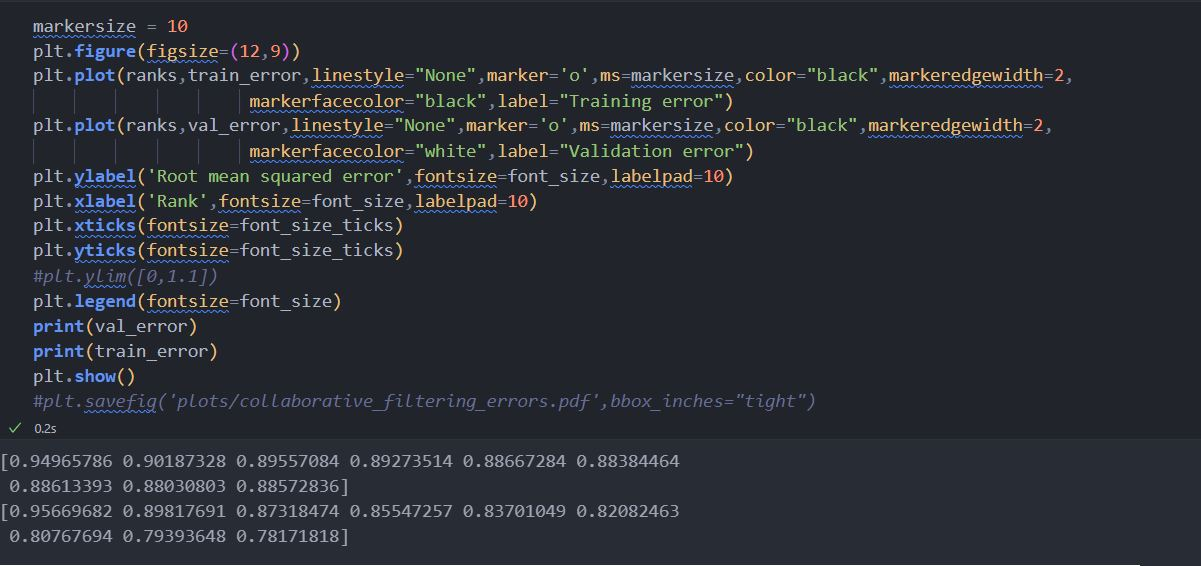
\includegraphics[width=20cm]{homework/homework_10/images/part_c_2.jpg}
\\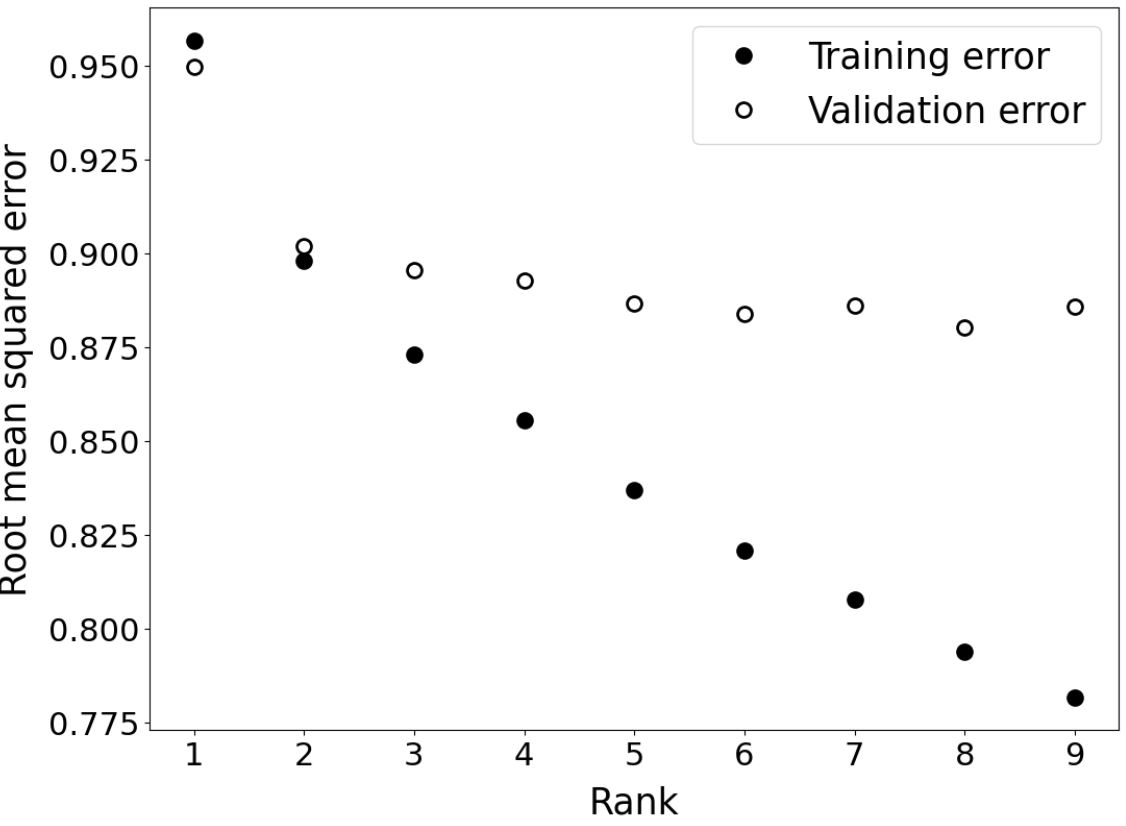
\includegraphics[width=15cm]{homework/homework_10/images/part_c_3.jpg}\\
\\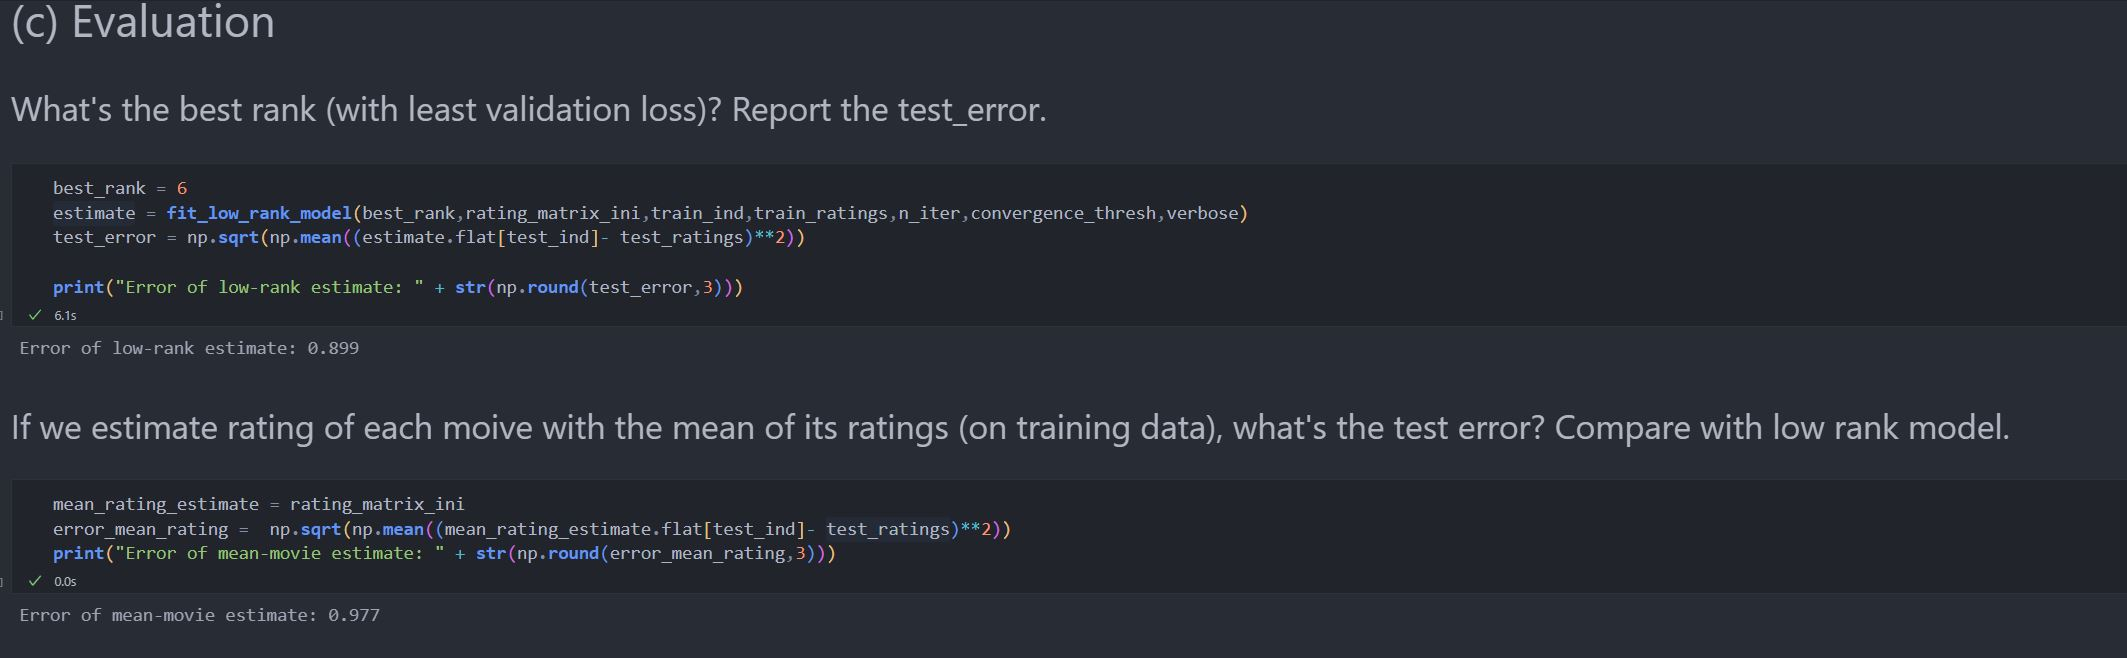
\includegraphics[width=20cm]{homework/homework_10/images/part _c.JPG}\\\includegraphics[width=20cm]
\\
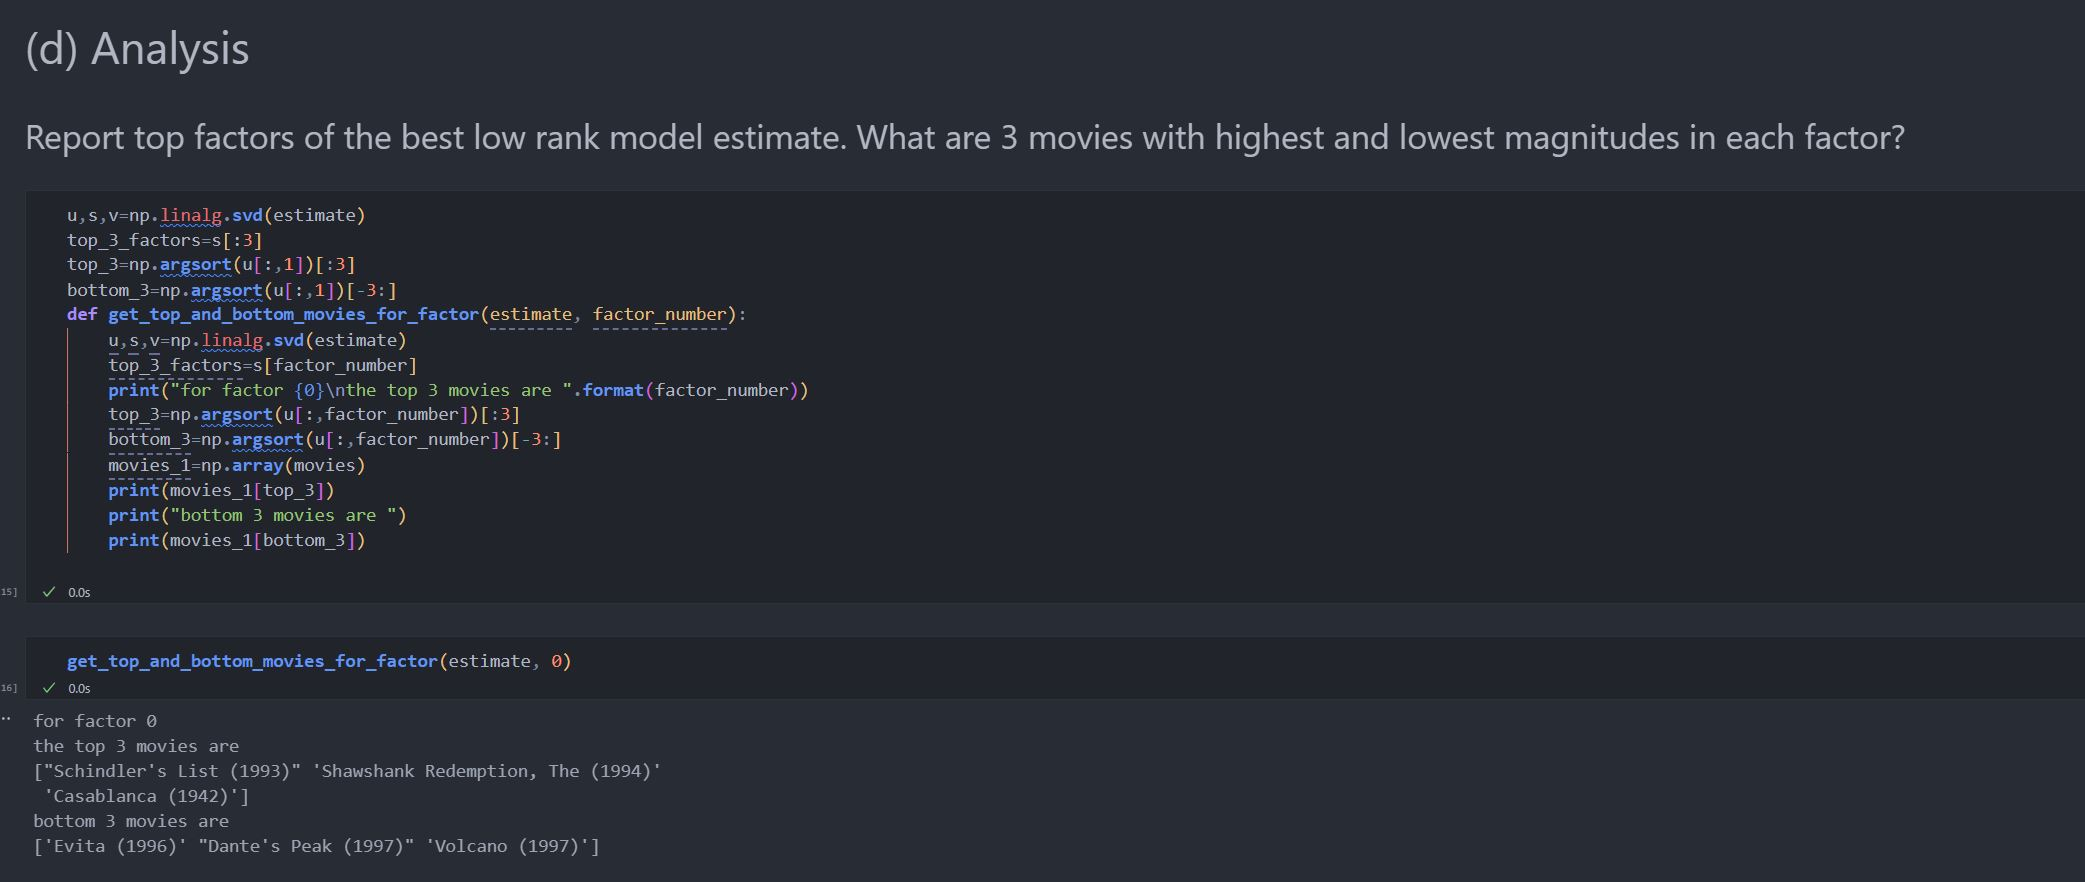
\includegraphics[width=20cm]{homework/homework_10/images/part d_1.jpg}
\end{itemize}
\end{enumerate}
 
\end{document}
